\documentclass[11pt,a4paper]{article}
\usepackage[margin=2.3cm]{geometry}
\usepackage[T1]{fontenc}
\usepackage{lmodern}
\usepackage{textcomp}
\usepackage{amsmath,amssymb,amsthm,bm}
\usepackage{booktabs}
\usepackage{graphicx}
\usepackage{xcolor}
\usepackage[hidelinks]{hyperref}
\usepackage{enumitem}
\setlist{itemsep=2pt}

\newcommand{\R}{\mathbb{R}}
\newcommand{\vr}{\mathbf{r}}
\newcommand{\vd}{\mathbf{d}}
\newcommand{\vw}{\mathbf{w}}
\newcommand{\G}{\Gamma}
\newcommand{\code}[1]{\texttt{#1}}
\newtheorem{proposition}{Proposition}

% all experimental numbers are generated from results/results.json
% generated by scripts/make_tex_tables.py — do not edit
\newcommand{\RealLadderTable}{
\begin{tabular}{lccccc}
\toprule
Model & MAPE & 95\,\% CI & median & $\delta{<}1.05$ & worst\\
\midrule
v1 original (reproduced exactly) & 10.08\,\% & 5.7--16.3 & 5.98\,\% & 37\,\% & 77\,\%\\
Pinhole + disparity offset (2 params) & 5.90\,\% & 4.3--7.7 & 5.09\,\% & 48\,\% & 16\,\%\\
Brown--Conrady, 18 params (same loss, FGLS) & 4.20\,\% & 2.8--5.8 & 3.04\,\% & 78\,\% & 14\,\%\\
$\Gamma$ grid + rotation, v2.0 loss & 5.64\,\% & 3.7--7.8 & 4.13\,\% & 56\,\% & 21\,\%\\
\quad + estimated noise model (FGLS) & 5.27\,\% & 3.4--7.4 & 3.91\,\% & 63\,\% & 22\,\%\\
\quad + radial prior ($\Gamma$ grid alone) & 4.58\,\% & 3.3--6.1 & 3.23\,\% & 67\,\% & 19\,\%\\
\quad + Brown--Conrady companion (\textbf{v2.1}) & \textbf{3.52\,\%} & 2.2--5.0 & 1.96\,\% & 74\,\% & 17\,\%\\
v2.1 without rig rotation & 4.86\,\% & 3.5--6.5 & 3.22\,\% & 59\,\% & 17\,\%\\
\bottomrule
\end{tabular}}

\newcommand{\SignificanceTable}{
\begin{tabular}{lccc}
\toprule
Comparison & $\Delta$ MAPE (pp) & $p$ & $p_\text{Holm}$\\
\midrule
v2.1 vs v1 & $-6.56$ & 0.0007 & 0.0035\\
v2.1 vs Brown--Conrady & $-0.68$ & 0.1676 & 0.4860\\
v2.1 vs $\Gamma$ alone & $-1.06$ & 0.0243 & 0.0970\\
$\Gamma$ alone vs Brown--Conrady & $+0.38$ & 0.6374 & 0.6374\\
$\Gamma$ + FGLS vs $\Gamma$ v2.0 loss & $-0.37$ & 0.1620 & 0.4860\\
\bottomrule
\end{tabular}}

\newcommand{\ParamTable}{
\begin{tabular}{lccc}
\toprule
Rig parameter & value & s.e.\ (sandwich) & s.e.\ (bootstrap)\\
\midrule
dx (m) & 0.2148 & 0.0060 & 0.0086\\
dy (m) & 0.0014 & 0.0020 & 0.0118\\
pitch ($^\circ$) & 0.254 & 0.071 & 0.242\\
yaw ($^\circ$) & 1.099 & 0.096 & 0.181\\
roll ($^\circ$) & -1.196 & 0.186 & 0.236\\
\bottomrule
\end{tabular}}

\newcommand{\SynBrownA}{
\begin{tabular}{lccccc}
\toprule
$\sigma=0.5$\,px, $N=$ & 15 & 30 & 60 & 120 & 480\\
\midrule
oracle (true cameras) & 0.16 & 0.15 & 0.16 & 0.15 & 0.15\\
\midrule
pinhole + offset & 3.90 & 3.95 & 3.71 & 3.82 & 3.51\\
v1 original & 12.02 & 8.63 & 8.60 & 7.32 & 6.74\\
pinhole + rotation & 2.81 & 2.54 & 2.95 & 2.23 & 2.44\\
Brown--Conrady & 1.86 & 0.58 & 0.36 & 0.28 & \textbf{0.18}\\
$\Gamma$ grid alone & \textbf{0.63} & \textbf{0.42} & 0.42 & 0.31 & 0.23\\
\textbf{v2.1 ensemble} & \textbf{0.63} & 0.45 & \textbf{0.36} & \textbf{0.27} & 0.18\\
\bottomrule
\end{tabular}}

\newcommand{\SynBrownB}{
\begin{tabular}{lccccc}
\toprule
$\sigma=2.0$\,px, $N=$ & 15 & 30 & 60 & 120 & 480\\
\midrule
oracle (true cameras) & 0.63 & 0.62 & 0.65 & 0.62 & 0.62\\
\midrule
pinhole + offset & 3.80 & 4.06 & 3.83 & 3.89 & 3.59\\
v1 original & 11.92 & 8.81 & 8.70 & 7.42 & 6.73\\
pinhole + rotation & 2.94 & 2.60 & 3.00 & 2.30 & 2.51\\
Brown--Conrady & 2.18 & 1.20 & 0.89 & 0.72 & 0.63\\
$\Gamma$ grid alone & \textbf{1.14} & \textbf{0.90} & \textbf{0.83} & \textbf{0.69} & 0.66\\
\textbf{v2.1 ensemble} & \textbf{1.14} & 1.02 & 0.84 & 0.69 & \textbf{0.63}\\
\bottomrule
\end{tabular}}

\newcommand{\SynFreeA}{
\begin{tabular}{lccccc}
\toprule
$\sigma=0.5$\,px, $N=$ & 15 & 30 & 60 & 120 & 480\\
\midrule
oracle (true cameras) & 0.16 & 0.16 & 0.16 & 0.15 & 0.15\\
\midrule
pinhole + offset & 4.49 & 4.27 & 3.98 & 4.09 & 3.77\\
v1 original & 11.85 & 8.57 & 8.55 & 7.25 & 6.61\\
pinhole + rotation & 3.32 & 3.04 & 3.43 & 2.65 & 2.87\\
Brown--Conrady & 1.58 & 0.79 & 0.55 & 0.44 & 0.34\\
$\Gamma$ grid alone & \textbf{0.72} & \textbf{0.58} & 0.54 & \textbf{0.35} & \textbf{0.26}\\
\textbf{v2.1 ensemble} & \textbf{0.72} & 0.65 & \textbf{0.48} & 0.36 & 0.27\\
\bottomrule
\end{tabular}}

\newcommand{\SynFreeB}{
\begin{tabular}{lccccc}
\toprule
$\sigma=2.0$\,px, $N=$ & 15 & 30 & 60 & 120 & 480\\
\midrule
oracle (true cameras) & 0.63 & 0.63 & 0.64 & 0.62 & 0.61\\
\midrule
pinhole + offset & 4.72 & 4.39 & 4.09 & 4.18 & 3.80\\
v1 original & 11.80 & 8.73 & 8.64 & 7.36 & 6.63\\
pinhole + rotation & 3.37 & 3.11 & 3.47 & 2.72 & 2.89\\
Brown--Conrady & 2.12 & 1.10 & 0.96 & 0.79 & 0.72\\
$\Gamma$ grid alone & \textbf{1.12} & \textbf{0.98} & \textbf{0.90} & 0.72 & \textbf{0.67}\\
\textbf{v2.1 ensemble} & \textbf{1.12} & 0.99 & 0.90 & \textbf{0.72} & 0.67\\
\bottomrule
\end{tabular}}

\newcommand{\CovOne}{85}
\newcommand{\CovTwo}{96}
\newcommand{\RmsZ}{0.80}
\newcommand{\ErrCorr}{0.55}
\newcommand{\DfEff}{15.1}
\newcommand{\NParams}{109}
\newcommand{\NFree}{107}
\newcommand{\SigmaLabel}{1.0}
\newcommand{\SigmaPx}{5.3}
\newcommand{\Kappa}{0.86}
\newcommand{\LamSel}{1}
\newcommand{\BudgetClick}{2.99}
\newcommand{\BudgetTotal}{3.13}
\newcommand{\MapeVOne}{3.52}
\newcommand{\MapeLegacy}{10.08}
\newcommand{\MedVOne}{1.96}
\newcommand{\MatchAcc}{77}
\newcommand{\MatchPrec}{96.1}
\newcommand{\MatchMed}{0.41}
\newcommand{\MatchMs}{15}

\providecommand{\MatchAcc}{n/a}\providecommand{\MatchPrec}{n/a}
\providecommand{\MatchMed}{n/a}\providecommand{\MatchMs}{n/a}
\providecommand{\SynBrownB}{}\providecommand{\SynFreeB}{}

\title{\textbf{Stereo Distance Measurement with a Per-Camera $\Gamma$-Grid Model}\\[4pt]
\large Mathematical Foundation and Evaluation (v2.1)}
\author{Gevorg}
\date{2026}

\begin{document}
\maketitle

\begin{abstract}
We measure metric distance from two calibrated cameras with a small, fully transparent
model. Each camera is a $5\times5\times2$ grid $\G$ of effective inverse focal lengths,
interpolated bilinearly over the image, and the rig is a baseline $\vd$ plus a relative
rotation $R(\bm\omega)$. We show that the $\G$ grid generalises radial lens distortion,
and regularise it towards a learned radial field. The noise model (click and label noise)
is estimated from the data and used for maximum-likelihood weighting, the regularisation
strength is chosen by repeated cross-validation, and the robust objective is minimised by
Levenberg--Marquardt with an analytic Jacobian. A Brown--Conrady model fitted to the same
points is averaged in as a companion. All gradients are derived by hand; no automatic
differentiation or SciPy is used. Under nested leave-one-out cross-validation on 27 real
points, the error falls from \MapeLegacy\,\% (version 1) to \textbf{\MapeVOne\,\%} MAPE
(median \MedVOne\,\%). This is close to the \BudgetTotal\,\% implied by the estimated
measurement noise alone. On simulated rigs with exact ground truth, the method approaches
the oracle error floor.
\end{abstract}

\tableofcontents
\newpage

%=====================================================================
\section{Pixel and normalised coordinates}
A pixel is $(u,v)$ on a $W\times H$ sensor ($2592\times1944$). With $(C_X,C_Y)=(W/2,H/2)$,
\begin{equation}
\tilde u = \frac{u-C_X}{C_X},\qquad \tilde v=\frac{v-C_Y}{C_Y}\qquad\in[-1,1].
\end{equation}

\section{The ray equation}
Every pixel defines a ray from the optical centre:
\begin{equation}\label{eq:ray}
\vr(u,v)=\begin{bmatrix}\tilde u\,\gamma_x(u,v)\\ \tilde v\,\gamma_y(u,v)\\ 1\end{bmatrix}.
\end{equation}
For an ideal pinhole with focal length $f$, $\gamma_x=C_X/f$ and $\gamma_y=C_Y/f$ everywhere. The nominal
value is $\G_0=[C_X/f_0,\ C_Y/f_0]$ with $f_0=2880$\,px. (Version 1 used one $\gamma$ for both axes; since
$C_X/C_Y=4/3$ this scaled every vertical ray component by $4/3$.)

\begin{proposition}[The $\G$ grid generalises radial distortion]\label{prop:radial}
Let a lens map undistorted normalised coordinates $\mathbf x_u$ to distorted ones by
$\mathbf x_d=\mathbf x_u\,D(\|\mathbf x_u\|)$ (radial distortion about the image centre, $D>0$ and
$\rho\mapsto\rho D(\rho)$ increasing). Then the exact ray of pixel $(u,v)$ has the form \eqref{eq:ray} with
\[
\gamma_x(u,v)=\frac{C_X}{f}\,g(r_d),\qquad \gamma_y(u,v)=\frac{C_Y}{f}\,g(r_d),\qquad
r_d=\frac{\sqrt{(u-C_X)^2+(v-C_Y)^2}}{f},
\]
for a single scalar function $g$ of the distorted radius.
\end{proposition}
\begin{proof}
$\mathbf x_d=((u-C_X)/f,(v-C_Y)/f)$ has norm $r_d=r_uD(r_u)$, which is invertible by monotonicity: $r_u=h(r_d)$.
Then $\mathbf x_u=\mathbf x_d/D(h(r_d))$. With $g:=1/(D\circ h)$ we get $x_u=\tilde u\,(C_X/f)\,g(r_d)$ and likewise
for $y$.
\end{proof}
So any radial lens is a \emph{radially symmetric} $\G$ field; tangential distortion and manufacturing
imperfections make it anisotropic and non-radial, which a grid can still follow. For
$D=1+k_1r^2+k_2r^4$, $g(r)=1-k_1r^2+(3k_1^2-k_2)r^4+O(r^6)$: this is the form of the radial prior
of \S\ref{sec:radial}.

\section{Bilinear interpolation}
Grid nodes sit at $u=j\,c_w$, $v=i\,c_h$ with $c_w=W/4$, $c_h=H/4$. With $f_x=u/c_w$, $f_y=v/c_h$, cell
$(i_y,i_x)=(\lfloor f_y\rfloor,\lfloor f_x\rfloor)$ (clamped) and $t_x=f_x-i_x$, $t_y=f_y-i_y$:
\begin{equation}\label{eq:bilinear}
\gamma(u,v)=\sum_{k=1}^{4}w_k\,\G_{n_k},\quad
\mathbf w=\big((1-t_x)(1-t_y),\;t_x(1-t_y),\;(1-t_x)t_y,\;t_xt_y\big).
\end{equation}
The weights sum to one, reproduce fields linear in $(u,v)$ exactly, make $\gamma$ continuous, and give
$\partial\gamma/\partial\G_{n_k}=w_k$. Noise-free experiments (\S\ref{sec:eval}) show that the $5\times5$ grid
represents a distorted lens to $0.06\,\%$ depth error, so the representation is not the limiting factor.

%=====================================================================
\section{Stereo geometry}
\subsection{Rig model and ray-space rectification}
For one 3-D point, $P_L=R(\bm\omega)P_R+\vd$ with $\vd=[d_x,d_y,0]^\top$ and
$R=R_z(\omega_\text{roll})R_y(\omega_\text{yaw})R_x(\omega_\text{pitch})$. The rig has about $1^\circ$ of yaw (a constant
61\,px disparity offset) and about $1^\circ$ of roll (vertical disparity linear in $u$). A multiplicative $\gamma$ can
produce neither. The right ray is rotated and perspective-normalised,
\begin{equation}\label{eq:rhat}
\vw=R\,\vr_R,\qquad \hat\vr_R=\vw/w_z,
\end{equation}
so that $Z\vr_L-Z'\hat\vr_R=\vd$ and, because $d_z=0$, $Z=Z'$:
\begin{equation}\label{eq:disp}
r_{L,x}-\hat r_{R,x}=\frac{d_x}{Z},\qquad r_{L,y}-\hat r_{R,y}=\frac{d_y}{Z}.
\end{equation}
The derivatives $\partial R/\partial\omega_j$ are products of the elementary rotations and one derivative
factor. They are exact, and checked against finite differences.

\subsection{Triangulation}
$A\mathbf x=\vd$ with $A=[\vr_L\;\;-\hat\vr_R]$, $\mathbf x=[Z,Z']^\top$ is solved by the normal equations
$A^\top A\mathbf x=A^\top\vd$ (closed-form $2\times2$ inverse, vectorised). The same problem is also solved by
batch gradient descent on $\|A\mathbf x-\vd\|^2$ with step $1/L$, $L=2\lambda_{\max}(A^\top A)$. Plain GD
contracts by $1-1/\kappa$ per step, and for distant points $\kappa$ reaches $10^3$--$10^4$, so Nesterov momentum
$\beta=(\sqrt\kappa-1)/(\sqrt\kappa+1)$ is used ($O(\sqrt\kappa)$ steps). The two agree to $10^{-8}$ (tested),
which is why OLS is the authoritative path. Since $Z=d_x/D$, $\partial Z/\partial D=-Z^2/d_x$: depth error
grows with $Z^2$.

%=====================================================================
\section{Loss function and noise model}
\subsection{Residuals}
\begin{equation}\label{eq:res}
e_x = D_x\frac{Z}{d_x}-1,\qquad e_y = D_y\frac{Z}{d_x}-\frac{d_y}{d_x},\qquad
D_{x,y}=r_{L,x/y}-\hat r_{R,x/y}.
\end{equation}
$e_x$ is the relative disparity error ($\approx$ relative depth error). It avoids the $Z^2$ gradient blow-up of a
$(Z_\text{pred}-Z)^2$ loss. $e_y$ is the epipolar misalignment in the same units.

\subsection{Noise model and maximum-likelihood weights}\label{sec:noise}
Two independent sources perturb a calibration point: click noise ($\sigma_\text{px}$ per coordinate), which
changes the ray-space disparity by $\sqrt2\sigma_\text{px}/f$; and label noise (the tape measurement), a relative
error $\sigma_\ell$. Propagating both through \eqref{eq:res},
\begin{equation}\label{eq:var}
\operatorname{Var}(e_x)\approx\sigma_\ell^2+c^2Z^2,\qquad \operatorname{Var}(e_y)\approx c^2Z^2,\qquad
c=\frac{\sqrt2\,\sigma_\text{px}}{f\,d_x}.
\end{equation}
Equal weighting of $e_x$ (version 2.0) is therefore maximum-likelihood only if label noise dominates.
Following feasible generalised least squares, we (i) fit with equal weights, (ii) estimate $c$ robustly from $e_y$
and $\sigma_\ell$ from the remainder of $e_x$ (median-absolute-deviation estimators, robust to mis-clicks), and
(iii) refit with residuals scaled by $1/\sigma_i$:
\begin{equation}
\tilde e_{x,i}=e_{x,i}\sqrt{\frac{\kappa^2+Z_\text{ref}^2}{\kappa^2+Z_i^2}},\qquad
\tilde e_{y,i}=e_{y,i}\frac{Z_\text{ref}}{Z_i},\qquad \kappa=\sigma_\ell/c,
\end{equation}
normalised at $Z_\text{ref}=\text{RMS}(Z)$ so the Huber threshold keeps its meaning. On the real data the
estimate is $\sigma_\ell=\SigmaLabel\,\%$, $\sigma_\text{px}=\SigmaPx$\,px, $\kappa=\Kappa$\,m. On synthetic data
with known noise, the estimator recovers both within 35\,\% (tested).

\subsection{Robust objective}
\begin{equation}\label{eq:loss}
\mathcal L=\frac1N\sum_{i=1}^{N}\Big[\rho_\delta(\tilde e_{x,i})+\lambda_y\,\rho_\delta(\tilde e_{y,i})\Big]
+\tfrac12(\theta-\theta_0)^\top H_\text{reg}(\theta-\theta_0),
\end{equation}
with the Huber function $\rho_\delta$ ($\delta=0.05$), $\lambda_y=0.5$, and the regulariser of \S\ref{sec:reg}.

%=====================================================================
\section{Priors, gauge and initialisation}\label{sec:reg}
\subsection{Hierarchical radial prior}\label{sec:radial}
Version 2.0 shrank $\G$ towards the constant $\G_0$ (anchor $\lambda_a$) and penalised its membrane energy
$\tfrac12\sum_{\text{edges}}(\G_i-\G_j)^2=\tfrac12\G^\top\mathbf L\G$ ($\mathbf L$: graph Laplacian). Every real lens has a
radial "bowl" (Prop.~\ref{prop:radial}), which this prior penalises, and that biases the fit when data are few.
Version 2.1 shrinks each camera's grid towards a \emph{learned} radial field:
\begin{equation}
\G_\text{prior}(n)=\G_0\big(1+a_1r_n^2+a_2r_n^4\big),\qquad
\mathcal R=\tfrac12\,\bm\delta^\top(\lambda_a I+\lambda_s\mathbf L)\bm\delta,\quad \bm\delta=\G-\G_0-B\mathbf a,
\end{equation}
where $r_n$ is the node's distorted radius and $B$ stacks $\G_0[r_n^2,r_n^4]$. $\mathcal R$ is an exact
quadratic form in $(\G,\mathbf a)$ with constant Hessian $M^\top(\lambda_aI+\lambda_s\mathbf L)M$, $M=[I,-B]$. The
coefficients $\mathbf a$ enter only the prior, never the rays, so inference and the file format are unchanged.
With little data $\G$ follows the two-parameter radial field; with more data it departs from it wherever the
data demand. This is the classical parametric model used as a prior mean for a non-parametric one.

\subsection{Gauge fixing}
Scaling every $\gamma$ and $d_x$ by one factor leaves \eqref{eq:disp} (almost) unchanged, so the centre node of
$\G_L$ is frozen at $\G_0$. $d_x$ is then the baseline expressed at $f_0$; depth is unaffected.

\subsection{Closed-form warm start}
Linearising $R\approx I+[\bm\omega]_\times$ with nominal $\G$ gives two equations per point that are linear in
$(d_x,d_y,\omega_p,\omega_y,\omega_r)$,
\[
r_{L,x}-r_{R,x}=d_x/Z+\omega_y-\omega_r\,r_{R,y},\qquad r_{L,y}-r_{R,y}=d_y/Z-\omega_p+\omega_r\,r_{R,x},
\]
solved by weighted least squares (DLT-style initialisation).

%=====================================================================
\section{Analytic gradients and Jacobian}
With $s=Z/d_x$ and $\mathbf a=\partial\mathcal L/\partial\hat\vr_{R,xy}$:
\begin{align}
&\frac{\partial e_x}{\partial\G_{L,n_k,x}}=s\,\tilde u_L\,w_k,\qquad \frac{\partial e_y}{\partial\G_{L,n_k,y}}=s\,\tilde v_L\,w_k,\\
&\frac{\partial\hat r_x}{\partial\vw}=\Big[\tfrac1{w_z},0,-\tfrac{w_x}{w_z^2}\Big],\quad
\frac{\partial\hat r_y}{\partial\vw}=\Big[0,\tfrac1{w_z},-\tfrac{w_y}{w_z^2}\Big],\quad
\frac{\partial\hat r}{\partial\vr_R}=\frac{\partial\hat r}{\partial\vw}R,\quad
\frac{\partial\hat r}{\partial\omega_j}=\frac{\partial\hat r}{\partial\vw}\frac{\partial R}{\partial\omega_j}\vr_R,\\
&\frac{\partial e_x}{\partial d_x}=-\frac{e_x+1}{d_x},\qquad \frac{\partial e_y}{\partial d_x}=-\frac{e_y}{d_x},\qquad
\frac{\partial e_y}{\partial d_y}=-\frac1{d_x},
\end{align}
and the right grid receives $-s\,(\partial\hat r/\partial\vr_R)_{x}\,\tilde u_R\,w_k$ (and the $y$ analogue). These give
both the gradient of $\mathcal L$ (for Adam) and the residual Jacobian $J$ (for Levenberg--Marquardt). All
components agree with central finite differences (largest relative discrepancy $10^{-7}$ for the gradient,
$5\cdot10^{-6}$ for $J$).

%=====================================================================
\section{Optimisation}
\subsection{Levenberg--Marquardt with IRLS (default)}
Multiplying \eqref{eq:loss} by $N$, each iteration solves
\begin{equation}
\big(J^\top WJ+N H_\text{reg}+\mu\operatorname{diag}\big)\bm\Delta=-\big(J^\top W\tilde{\mathbf e}+N H_\text{reg}(\theta-\theta_0)\big),
\end{equation}
where $W$ holds the Huber IRLS weights $\min(1,\delta/|\tilde e|)$ and $\lambda_y$. A step is accepted only if the
objective decreases ($\mu\leftarrow0.3\mu$), otherwise $\mu\leftarrow5\mu$, so the method is monotone. A fit on 27 points
takes about 0.04\,s.

\subsection{Adam}
Adam with bias correction, per-block learning rates and cosine decay minimises the same objective. On the
identical objective, both optimisers reach the same minimum to $10^{-10}$ relative (Fig.~\ref{fig:conv}, and
tested), and the gradient vanishes at the LM solution ($<10^{-7}$). Two independent methods agreeing certifies
convergence.

\begin{figure}[h]\centering
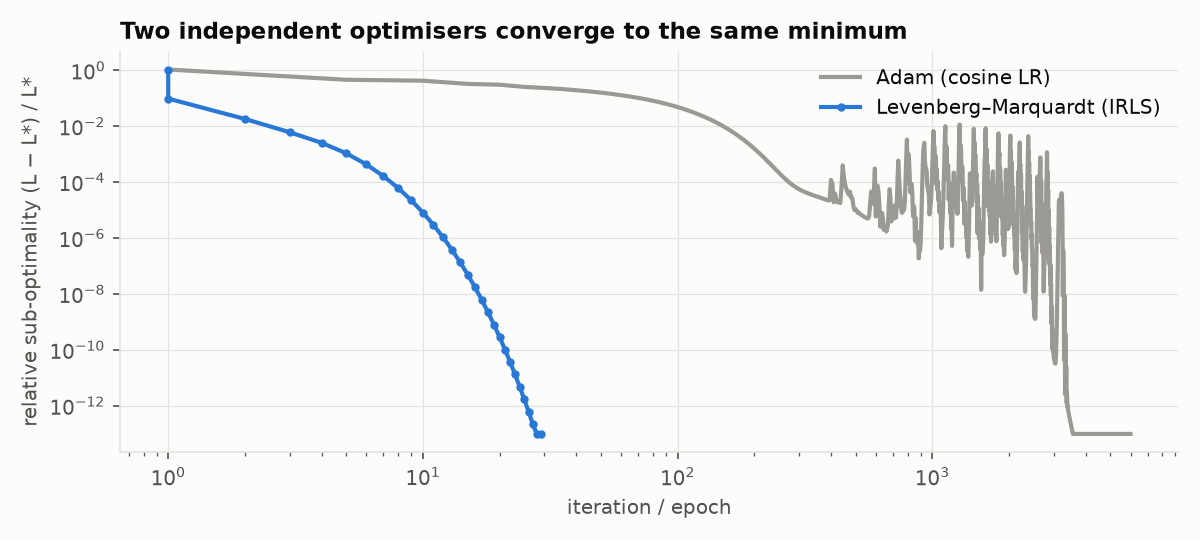
\includegraphics[width=0.8\linewidth]{figures/convergence.png}
\caption{Relative sub-optimality of LM and Adam on the same objective.}\label{fig:conv}
\end{figure}

%=====================================================================
\section{Model selection and model averaging}
\subsection{Regularisation strength by repeated cross-validation}
Noise-free experiments show that the best $\lambda_s$ depends strongly on $N$ and the noise level, so it cannot be
fixed. \code{train} selects $\lambda_s\in\{0.01,\dots,3\}$ by 5-fold cross-validation repeated over 3 shuffles
(held-out depth MAPE; ties go to the stronger penalty), using \emph{only its training points}. Evaluating this
procedure by leave-one-out is therefore a \emph{nested} cross-validation (Varma \& Simon 2006): no hyper-parameter
ever sees the test point. On all 27 points it selects $\lambda_s=\LamSel$.

\subsection{Averaging with a Brown--Conrady companion}
The standard parametric alternative is the Brown--Conrady model used by OpenCV. Per camera it has a focal
length, a principal point, radial $k_1,k_2$ and tangential $p_1,p_2$, plus the same rotation and baseline (18
parameters, $f_L=f_0$ as gauge). It is fitted with \emph{the same residuals, Huber loss and noise model}. Its
out-of-sample errors correlate with the $\G$ grid's at only $\rho=\ErrCorr$. For two unbiased predictors of equal
error variance $\sigma^2$, the equal-weight average has variance $\tfrac{\sigma^2}{2}(1+\rho)$ (Bates \& Granger 1969).
Averaging therefore reduces error unless $\rho\approx1$. v2.1 reports the equal-weight average of both depths. The
weights are fixed in advance, not fitted, so the averaging introduces no selection bias. The $\G$ grid remains the
geometric engine (epipolar curves, matching, uncertainty).

%=====================================================================
\section{Diagnostics}
\paragraph{Effective degrees of freedom.} For the penalised fit, $\text{df}=\operatorname{tr}\big[(J^\top WJ+NH_\text{reg})^{-1}J^\top WJ\big]$
(the trace of the hat matrix). The model has \NParams\ parameters (\NFree\ free), but df $=\textbf{\DfEff}$: the
data determine about fifteen directions in parameter space, and the priors fix the rest.
\paragraph{Parameter uncertainty.} The sandwich covariance $A^{-1}(\sigma_x^2J_x^\top W_xJ_x+\sigma_y^2J_y^\top W_yJ_y)A^{-1}$
is compared with a 200-sample nonparametric bootstrap:
\begin{center}\ParamTable\end{center}
The two agree for $d_x$, yaw and roll. For $d_y$ and pitch, which are identified only by the heavy-tailed vertical
residuals, the sandwich estimate is optimistic; the bootstrap values should be quoted.

%=====================================================================
\section{Epipolar geometry and correspondence search}
For a left pixel and depth $Z$: $P_R=R^\top(Z\vr_L-\vd)$, then $\G_R$ is inverted by the fixed point
$u\leftarrow C_X+C_Xt_x/\gamma_x(u,v)$. Sweeping $1/Z$ traces the curved, tilted epipolar curve. Along it, zero-mean
normalised cross-correlation ($31\times31$ patches, every pixel) is maximised and refined with the parabola
$\Delta=(s_{-1}-s_{+1})/(2(s_{-1}-2s_0+s_{+1}))$. A match is accepted only if its ZNCC is $\ge0.6$, the template is
textured, and the reverse search along the \emph{left} epipolar curve returns within 2\,px of the click (a
left--right consistency check). Accepted matches are refined by inverse-compositional Lucas--Kanade. Images
are pre-processed by CLAHE with bilinear blending between tiles.

%=====================================================================
\section{Uncertainty of a measurement}
Click noise is propagated to first order through the complete model, and the model's relative prediction error
$\varepsilon$ (from the cross-validation inside training) is added in quadrature:
\[
\sigma_Z^2=\sum_{p\in\{u_L,v_L,u_R,v_R\}}\Big(\frac{\partial Z}{\partial p}\Big)^2\sigma_\text{px}^2+(\varepsilon Z)^2 .
\]
Out of sample, $|Z-Z_\text{true}|\le\sigma_Z$ holds for \CovOne\,\% of points (Gaussian ideal 68\,\%) and $\le2\sigma_Z$
for \CovTwo\,\% (ideal 95\,\%), with RMS $z$-score \RmsZ. The interval is conservative at $1\sigma$ because the
errors are heavy-tailed, and well calibrated at $2\sigma$.

%=====================================================================
\section{Evaluation}\label{sec:eval}
\subsection{Protocol}
With $N=27$ labelled points all real-data numbers are nested leave-one-out cross-validation. Confidence intervals
come from 4000 bootstrap resamples. Paired comparisons use a two-sided sign-flip permutation test (20\,000
draws, no normality assumption) with Holm's correction for the five comparisons.

\subsection{Real dataset}
\begin{center}\small\RealLadderTable\end{center}

\begin{center}\small\SignificanceTable\end{center}

v2.1 is significantly better than version 1. Among the modern models the differences are not significant with
27 points; they are resolved by the controlled benchmark below. Removing the rig rotation costs over one
percentage point.

\paragraph{Error budget.} The noise model estimated from the data predicts \BudgetClick\,\% MAPE from click noise
alone and \BudgetTotal\,\% with label noise, against the observed \MapeVOne\,\%. Most of the remaining error is
therefore measurement noise in the calibration data, not model error. Further gains on this rig require better
data (Section~\ref{sec:limits}).

\begin{center}
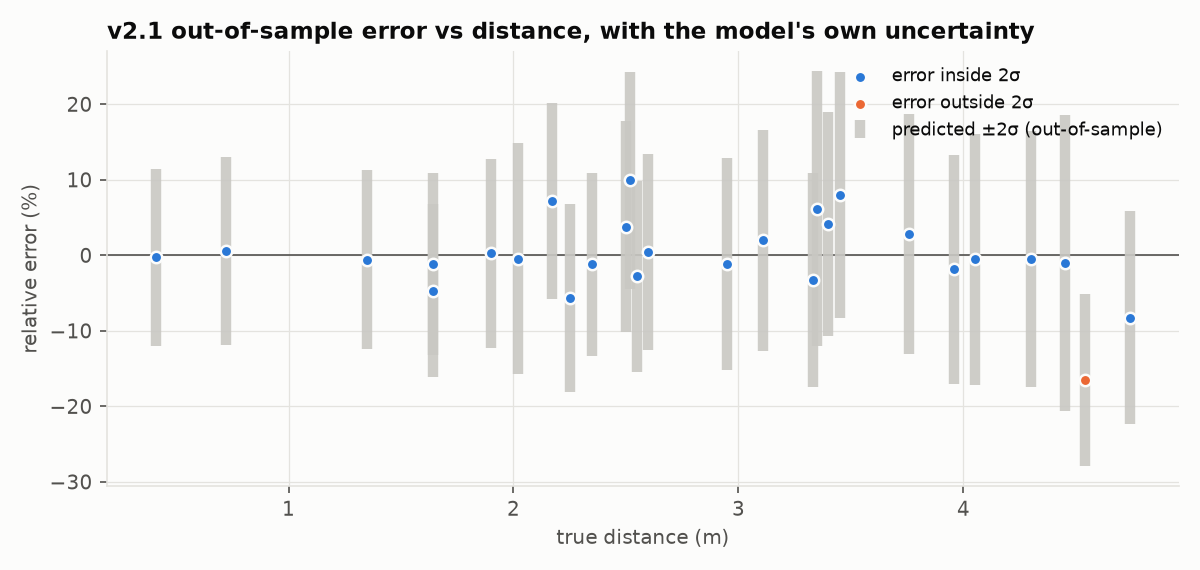
\includegraphics[width=0.85\linewidth]{figures/error_vs_distance.png}
\end{center}

\subsection{Controlled synthetic benchmark}
Two simulated rigs have exact ground truth: a Brown--Conrady lens (the baseline's own model family), and a
free-form lens that adds decentering and a smooth non-radial waviness of $\pm4$\,px. Both have unequal focal
lengths, off-centre principal points, a 0.20\,m baseline and a $(0.15^\circ,0.9^\circ,-1.1^\circ)$ rotation.
Training points carry click noise $\sigma$ and 1\,\% label noise; 500 fresh points per seed are scored.
The \emph{oracle} triangulates with the true cameras, so its error is the floor set by the test clicks' own noise.
Held-out MAPE (\%), best fitted model in bold:

\begin{center}\small
\textit{Brown--Conrady lens}\par\smallskip
\SynBrownA\par\medskip
\SynBrownB\par\bigskip
\textit{Free-form lens}\par\smallskip
\SynFreeA\par\medskip
\SynFreeB
\end{center}

\begin{center}
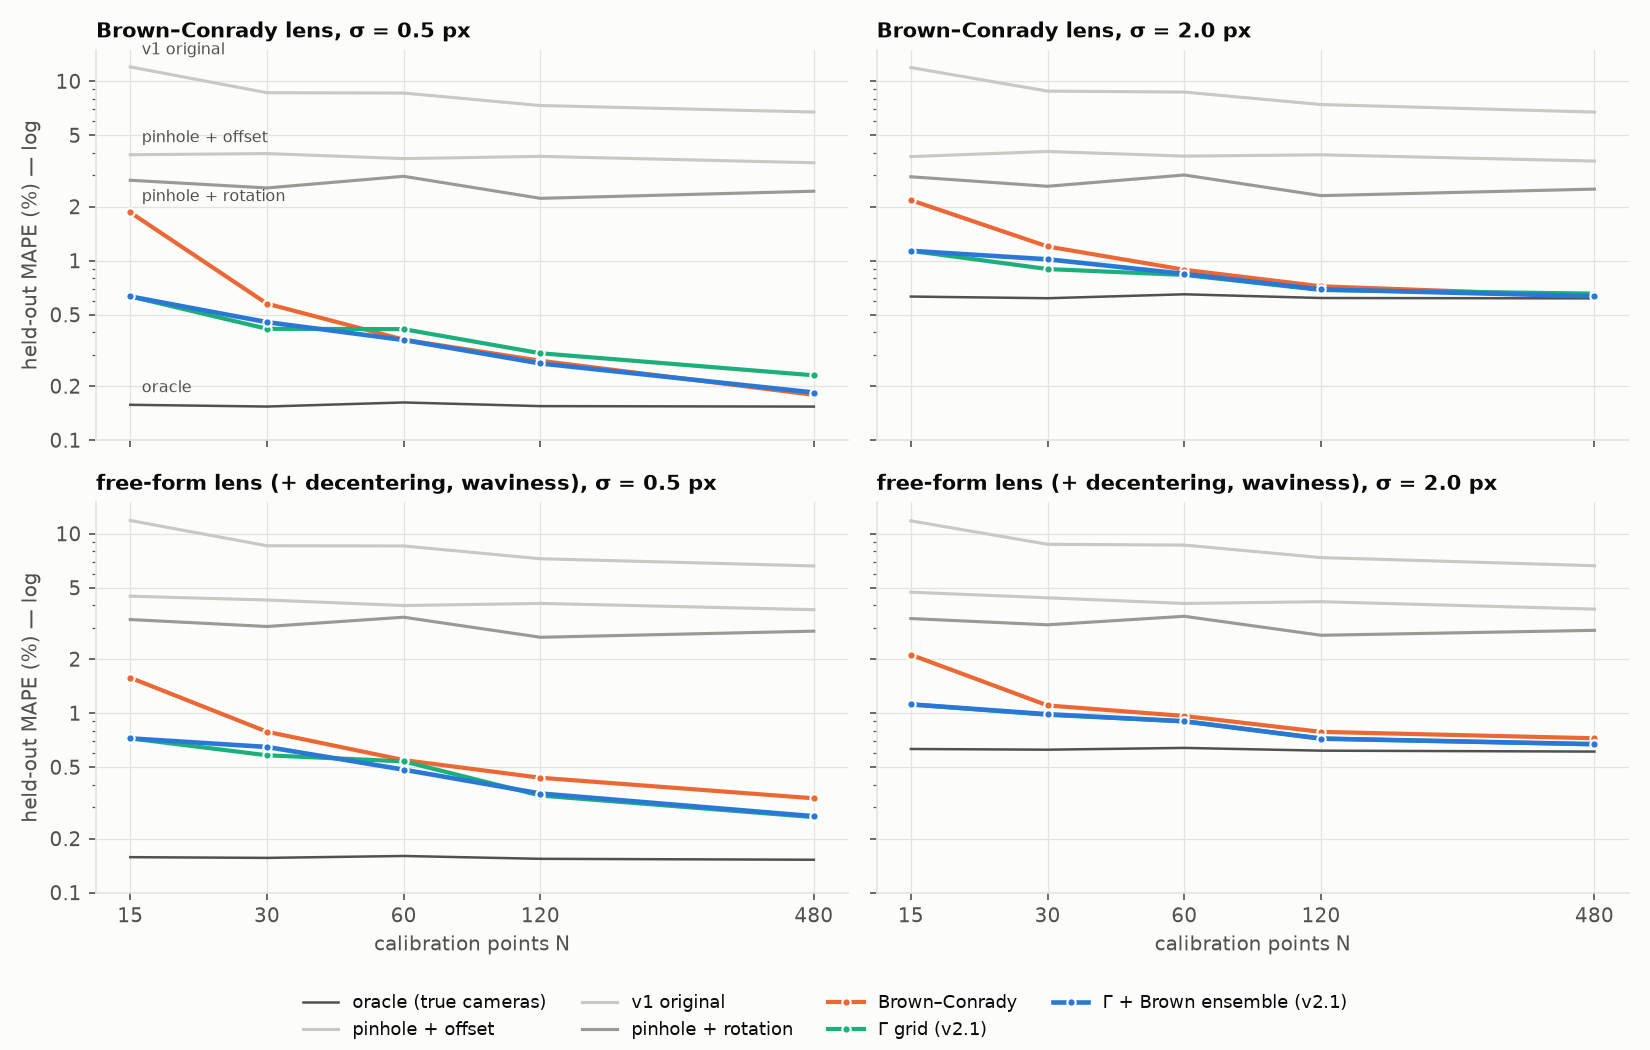
\includegraphics[width=\linewidth]{figures/synthetic_benchmark.png}
\end{center}

\subsection{Automatic matching}
On a ray-traced scene seen through the simulated rig, 200 random clicks: \MatchAcc\,\% are accepted by ZNCC +
left--right check; \MatchPrec\,\% of those are within 3\,\% of the true depth (median error \MatchMed\,\%);
\MatchMs\,ms per click.

%=====================================================================
\section{Complexity and numerical safeguards}
Ray evaluation and triangulation are $O(1)$. One LM iteration costs $O(NP^2+P^3)$ with $P=109$ (well under a
millisecond). A full training run (noise model, 90 inner fits for $\lambda_s$, companion) takes about 3\,s, and nested
LOOCV about 2\,min. Safeguards: near-singular $A^\top A$ falls back to $Z=d_x/D$; $D\le0$ or $Z\le0$ gives NaN;
$\G\in[0.05,5]$ and $d_x\ge0.02$\,m; LM only accepts decreasing steps; trial steps that make the Brown--Conrady
undistortion diverge are rejected.

\section{Limitations and future work}\label{sec:limits}
\begin{itemize}
\item \textbf{Data.} The error budget shows that the 27 hand-clicked points, with estimated $\sigma_\text{px}\approx\SigmaPx$\,px
and $\sigma_\ell\approx\SigmaLabel\,\%$, limit accuracy. A calibration board at measured distances would give hundreds
of sub-pixel points; the synthetic results suggest errors near 0.3\,\% would then be reachable.
\item Model differences below about one percentage point cannot be resolved with 27 points (the CIs are about $\pm1.5$\,pp).
\item Bundle adjustment (using correspondences without known distance) and multi-scale grids are natural extensions.
\end{itemize}

%=====================================================================
\appendix
\section{Mapping between code and mathematics}
\begin{center}\small
\begin{tabular}{ll}
\toprule
Function (package \texttt{stereo\_gamma}) & Implements\\
\midrule
\code{geometry.bilinear\_weights}, \code{rays} & eqs.~\eqref{eq:bilinear}, \eqref{eq:ray}\\
\code{geometry.rotation\_with\_jacobians}, \code{right\_rays\_in\_left} & $R$, $\partial R/\partial\omega$, eq.~\eqref{eq:rhat}\\
\code{model.StereoModel.triangulate\_gamma}, \code{triangulate\_gd} & OLS; batch GD + Nesterov\\
\code{model.StereoModel.triangulate} & v2.1 ensemble depth\\
\code{model.StereoModel.depth\_uncertainty} & error propagation\\
\code{training.objective}, \code{solver.residual\_jacobian} & eq.~\eqref{eq:loss}, gradient and $J$\\
\code{training.estimate\_noise}, \code{noise\_scales} & noise model, eq.~\eqref{eq:var}\\
\code{solver.regulariser\_hessian}, \code{radial\_basis} & anchor, membrane, radial prior\\
\code{solver.levenberg\_marquardt}, \code{training.Adam} & optimisers\\
\code{training.select\_smoothing} & repeated $k$-fold selection of $\lambda_s$\\
\code{solver.diagnostics} & effective df, sandwich covariance\\
\code{baselines.BrownConradyStereo} & parametric companion / baseline\\
\code{matching.epipolar\_match}, \code{lk\_refine}, \code{clahe} & correspondence search\\
\code{evaluation.loocv}, \code{coverage}, \code{signflip\_test} & evaluation protocol\\
\code{legacy.train\_legacy} & exact re-implementation of version 1\\
\code{synthetic.SyntheticRig.triangulate} & oracle\\
\bottomrule
\end{tabular}
\end{center}

\section*{References}
\small
\begin{enumerate}[label={[\arabic*]}]
\item R.~Hartley, A.~Zisserman. \emph{Multiple View Geometry in Computer Vision}, 2nd ed., CUP, 2004.
\item Z.~Zhang. A flexible new technique for camera calibration. \emph{IEEE TPAMI} 22(11), 2000.
\item D.~C.~Brown. Decentering distortion of lenses. \emph{Photogrammetric Engineering} 32(3), 1966.
\item P.~J.~Huber. Robust estimation of a location parameter. \emph{Ann. Math. Statist.} 35(1), 1964.
\item P.~W.~Holland, R.~E.~Welsch. Robust regression using iteratively reweighted least-squares. \emph{Commun. Stat.} 6(9), 1977.
\item J.~J.~Mor\'e. The Levenberg--Marquardt algorithm: implementation and theory. \emph{Numerical Analysis}, LNM 630, 1978.
\item B.~Triggs, P.~McLauchlan, R.~Hartley, A.~Fitzgibbon. Bundle adjustment --- a modern synthesis. \emph{Vision Algorithms}, 2000.
\item D.~P.~Kingma, J.~Ba. Adam: a method for stochastic optimization. \emph{ICLR}, 2015.
\item Y.~Nesterov. A method for solving the convex programming problem with convergence rate $O(1/k^2)$. \emph{Soviet Math. Dokl.} 27, 1983.
\item T.~Hastie, R.~Tibshirani. \emph{Generalized Additive Models}. Chapman \& Hall, 1990 (effective degrees of freedom).
\item S.~Varma, R.~Simon. Bias in error estimation when using cross-validation for model selection. \emph{BMC Bioinformatics} 7, 2006.
\item J.~M.~Bates, C.~W.~J.~Granger. The combination of forecasts. \emph{Oper. Res. Q.} 20(4), 1969.
\item S.~Holm. A simple sequentially rejective multiple test procedure. \emph{Scand. J. Statist.} 6(2), 1979.
\item B.~Efron, R.~Tibshirani. \emph{An Introduction to the Bootstrap}. Chapman \& Hall, 1993.
\item B.~D.~Lucas, T.~Kanade. An iterative image registration technique with an application to stereo vision. \emph{IJCAI}, 1981.
\item S.~Baker, I.~Matthews. Lucas--Kanade 20 years on: a unifying framework. \emph{IJCV} 56(3), 2004.
\item K.~Zuiderveld. Contrast limited adaptive histogram equalization. \emph{Graphics Gems IV}, 1994.
\item H.~Hirschm\"uller. Stereo processing by semiglobal matching and mutual information. \emph{IEEE TPAMI} 30(2), 2008.
\end{enumerate}
\end{document}
